\chapter{Popis softvéru}\label{chap:popis}

V predchádzajúcich kapitolách sme spravili prehľad problematiky a algoritmov, 
ktoré slúžia na hľadanie minimálnej dominujúcej množiny. V tejto kapitole sa 
venujeme popisu a návrhu softvéru, ktorý slúži na porovnanie týchto algoritmov 
a otestovanie týchto algoritmov v praxi.


\section{Analýza existujúcich riešení}

Keďže problém nájdenia minimálnej dominujúcej množiny je podobný problému 
vrcholového pokrytia je často súčasťou aplikácií venujúcim sa zhromažďovaniu 
rôznych grafových algoritmov. Veľa nám známych z nich obsahuje iba základy 
výpočet všetkých možností, alebo jednoduchý aproximačný algoritmus, preto 
tu uvedieme iba jedného zástupcu tohto druhu. Popri vyvíjaní nášho 
softvéru sme pracovali aj s nástrojmi pre analýzu grafov. Tieto sa taktiež 
zväčša vyskytujú v balíkoch s inými nástrojmi pracujúcimi s grafmi (napr. 
vizualizácia). Uvedieme tiež iba jedného zástupcu.

% \todo{
% Cieľom tejto etapy je oboznámenie sa s prostredím, v ktorom bude aplikácia používaná. 
% Dôraz sa kladie na hlbšie pochopenie interakcie aplikácie s prostredím. 
% Ak existujú, treba vykonať aj analýzu podobných systémov.
% }

\subsection{Network Benchmark}

Reprezentantom softvérov na analýzu grafov je Network Benchmark. Ide o softvér, 
ktorý získal podporu aj Alberta Barabásiho. Bol vyvíjaný v rokoch 2005 až 2011. 
Obsahuje príklady, dokumentáciu a podklady k práci s analýzou grafu. Je 
naprogramovaný v jazyku \Java\ a k jeho silným stránkam patrí relatívna 
prehľadnosť pri veľkom množstve nastaveniach a možnostiach analýzy. 

Je dostupný na adrese: \url{http://nwb.cns.iu.edu/index.html}

\begin{figure}
	\centering
	\greybox{%
		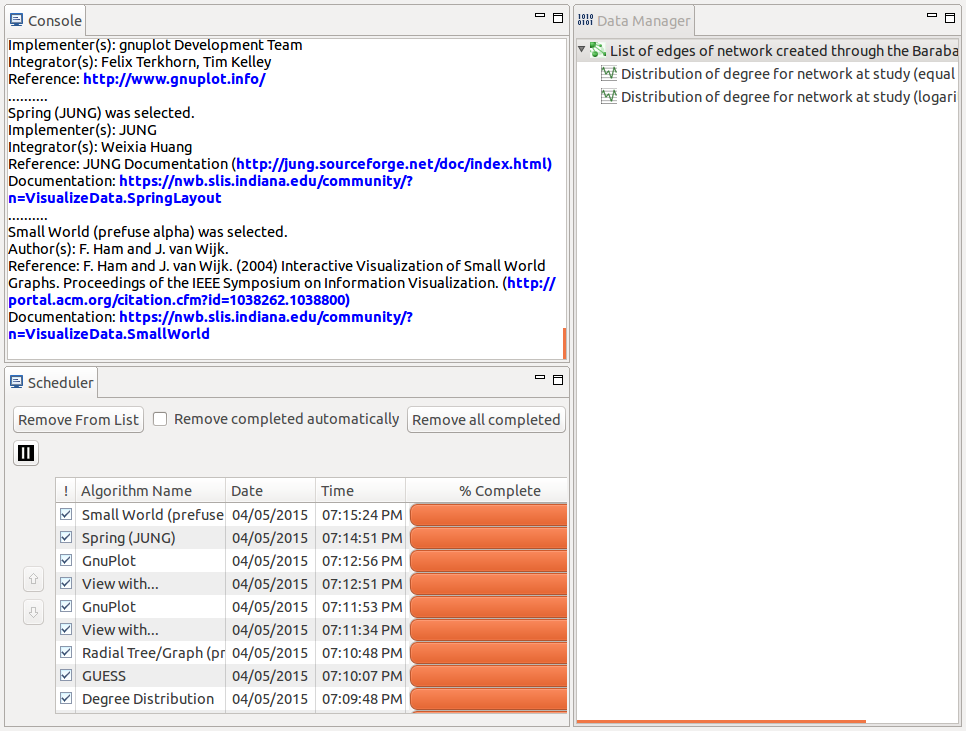
\includegraphics[scale=0.3]{obrazky/nwb1}%
	}
	\caption{\emph{Softvér Network Benchmark.} V ľavej hornej časti 
		obrazovky sa nachádzajú výpisy. V dolnej prebiehajúce a ukončené 
		akcie a výpočty. Vpravo sú zhromaždené výsledky výpočtov.}
	\label{img:vis:nwb1}
\end{figure}

\begin{figure}
	\centering
	\greybox{%
		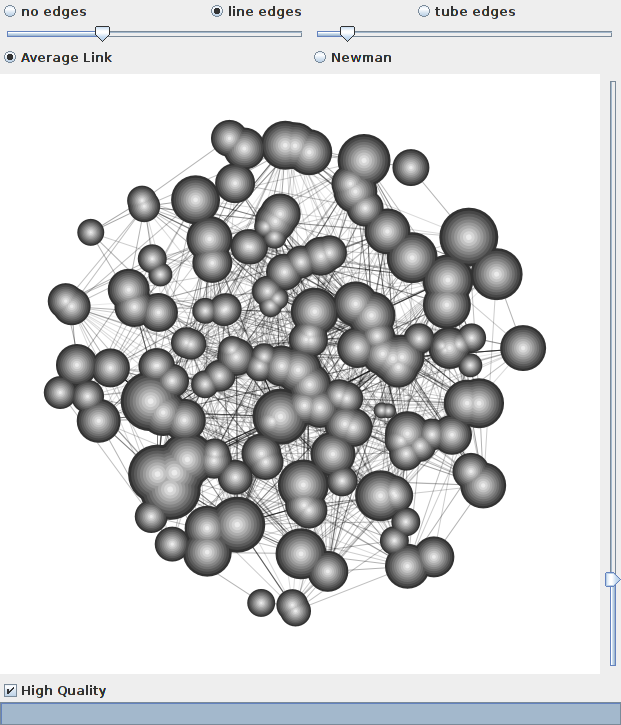
\includegraphics[scale=0.3]{obrazky/nwb2}%
	}
	\caption{\emph{Softvér Network Benchmark.} Tu je zobrazená vizualizácia 
		siete malého sveta. Bublinky znázorňujú jednotlivé klastre.}
	\label{img:vis:nwb2}
\end{figure}

Na obrázku \ref{img:vis:nwb1} je vidno hlavnú obrazovku aplikácie. Práca s 
aplikáciou prebieha tradične tak, že používateľ načíta nejakú grafovú štruktúru, 
následne sa mu zobrazí v stĺpci napravo, označí ju a z bohatej ponuky zvolí 
nejakú analýzu. Vľavo dole, potom vidí priebeh jeho akcií a vľavo hore bližšie 
popisy toho, čo sa práve vykonáva.


\subsection{NetworkX}

Tento softvér je reprezentantom zbierky rôznych algoritmov na grafoch. Je 
vyvíjaný od roku 2005 až doteraz. Posledná stabilná verzia v čase písania 
tejto práce je zo septembra roku 2014. Ide o rozšírenie jazyka Python o novú 
knižnicu.

Sídlo projektu je na adrese: \url{https://networkx.github.io/}

\begin{figure}
	\centering
	\greybox{%
		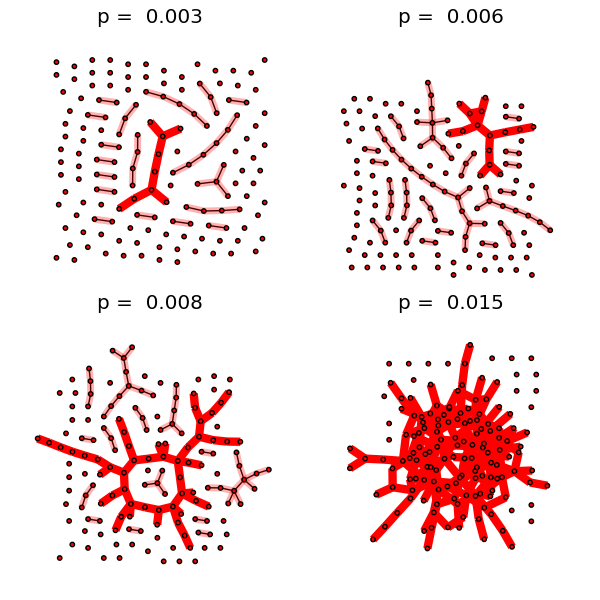
\includegraphics[scale=0.6]{obrazky/nx}%
	}
	\caption{\emph{Softvér NetworkX.} Tu je zobrazená vizualizácia 
		náhodného grafu s rôznymi pravdepodobnosťami hrán.}
	\label{img:vis:nx}
\end{figure}

Na obrázku \ref{img:vis:nx} je znázornená vizualizácia so softvérom NetworkX. 
Ide o tvorbu náhodného grafu pomocou určenia pravdepodobnosti vzniku hrany. 
Vidno, že aj keď je NetworkX hlavne zbierkou algoritmov, poskytuje peknú 
vizualizáciu. Jeho nedostatkom pre nás je, že na riešenie problému hľadania 
minimálnej dominujúcej množiny poskytuje iba pažravý algoritmus.

\section{Špecifikácia požiadaviek}

Ako vidno, súčasné softvéry majú dobrú ponuku rôznych algoritmov a veľa 
odlišných vizualizácií. Avšak daň za to, že ponúkajú riešenie na veľa problémov 
je tá, že zväčša je dostupný iba jeden algoritmus na riešenie.

Keďže sa my v práci zaoberáme porovnávaním algoritmov, veľmi nám táto 
skutočnosť nesedí. Preto by sme mali navrhnúť vlastný softvér, ktorý zrejme 
nebude poskytovať riešenia na veľa problémov ale veľa riešení na jeden problém.

%\todo{Čo očakávame od softvéru a prečo je viac fajn ako konkurencia.}

\subsection{Požiadavky}

\todo{Čo má softvér robiť z hladiska funkčnosti.}

\subsection{Prevádzkové požiadavky}

\todo{Čo má softvér robiť z hladiska hardvéru.}

% \todo{
% Východiskom tejto etapy je etapa analýzy. 
% Zaoberá sa úlohami, ktoré má aplikácia zabezpečiť. 
% Oboznámime sa s prostredím, v ktorom bude aplikácia používaná. 
% Zaujímame sa o to, čo chce zadávateľ riešiť, čo požaduje, aby aplikácia vykonávala a pre koho je určená. 
% Zatiaľ nás nezaujíma spôsob realizácie.  
% Cieľom špecifikácie požiadaviek je stanovenie služieb, ktoré zákazník požaduje od systému a ohraničenia na jeho vývoj a prevádzku. 
% Teda zaujímame sa o funkcionálnu stránku systému, potom o to, aké by mali byť vstupy a výstupy systému 
% a s akými údajmi systém bude pracovať, potom o prevádzkové požiadavky 
% (počet a charakteristika používateľov, časová odozva systému, potrebný hardvér a softvér, bezpečnosť a ochrana systému a iné potrebné požiadavky). 
% Prevádzkové požiadavky nazývame aj nefunkcionálne požiadavky. 
% Detailný opis špecifikácie požiadaviek na softvér  najdeme v (1) alebo v štandarde IEEE 830.
% }

\section{Návrh}

\todo{Stručný opis, čo chceme dosiahnuť.}

% vzťahy medzi časťami softvéru, 
%štruktúru dát a rozhranie systému.

\subsection{Technické požiadavky}

\todo{Self-descripting}

\subsection{Používateľské požiadavky}

\todo{Self-descripting}

\subsection{Použité technológie a návrhové vzory atď.}

\todo{Self-descripting}

%Keďže projekt bol pokračovaním predošlej práce za hlavný programovací jazyk 
%bola zvolená \Java. Na grafické znázornenie sú to jednotlivé triedy balíkov 
%AWT a Swing. Na generovanie náhodných reťazcov sme použili špeciálne upravenú 
%triedu s návrhovým vzorom \emph{singleton}. Vďaka celkovej nenáročnosti na 
%technológie a zameraniu projektu nebolo potrebné použiť viac technológií.

\subsection{Rozhranie aplikácie}

\todo{Vstup/výstup -- aj pre jednotlivé časti softvéru}

%Rozhranie vizualizácií bolo podobné ako všetkých iných štruktúr 
%implementovaných v~predošlej verzií softvéru. Vstupné dáta boli zadávané do 
%vstupného textového poľa, alebo klikaním myšou. Podľa stlačeného tlačidla sa 
%spustil daný proces. Výstupne údaje boli prezentované vo vykresľovacom okne 
%pre dátovú štruktúru a vo výpise pre komentáre. Vykreslená štruktúra sa dala 
%zväčšiť, zmenšiť a posunúť pomocou myšky.

%Pre každú dátovu štruktúru bolo potrebné zabezpečiť vstupné textové pole, 
%prípadne dodatočné vstupné metódy a tlačidlá pre všetky operácie.

% \todo{
% V tejto etape sa ujasňuje koncepcia systému. 
% Navrhne sa jeho dekompozícia, určia sa vzťahy medzi časťami systému a ohraničenia funkcionality. 
% Túto časť návrhu zvyčajne modelujeme technikami softvérového inžinierstva napr. procesným modelom DFD (Data Flow Diagram, str.24 v (1)) 
% Dekompozícia sa môže urobiť aj na základe iných princípov ako je funkcionálny (str. 53 v (1)). 
% V ďalšom sa identifikuje štruktúra údajov, ktoré do systému vstupujú, ktoré systém spracováva a produkuje. 
% Vzťah medzi údajmi sa modeluje entitno-relačným diagramom, v ktorom sa pomenovávajú vzťahy medzi údajovými entitami. 
% Ak použijeme model DMD (Data Model Diagram), potom v ňom znázorňujeme kvantifikované vzťahy dohodnutými značkami na označenie kardinality. 
% Ak rozložíme vzťah typu M:N pomocou väzobnej entity, potom dostávame fyzický model údajov.  (str.31 v (1))
% V etape návrhu sa navrhne rozhranie systému ( čo do systému vstupuje a čo z neho vystupuje), 
% navrhne sa typ používateľského rozhrania (príkazovo orientované rozhranie, menu, priame riadenie, komunikácia v prirodzenom jazyku ), 
% plán realizácie systému a stanovia sa podmienky, za akých bude používateľ akceptovať produkt. 
% Odhadnú sa potrebné ľudské a materiálne zdroje a navrhne sa postup zaškolovania používateľov.
% }

